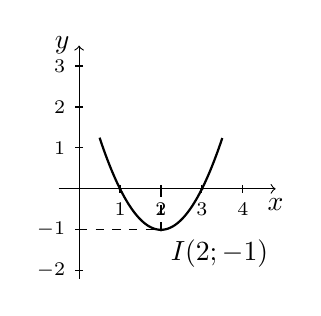
\begin{tikzpicture}[scale=0.52]
    \draw[->] (-0.5,0) -- (4.8,0) node[below] {$x$};
    \draw[->] (0,-2.2) -- (0,3.5) node[left] {$y$};

    \foreach \x in {1,2,3,4}
        \draw (\x,0.1) -- (\x,-0.1) node[below] {\scriptsize $\x$};

    \foreach \y in {-2,-1,1,2,3}
        \draw (0.1,\y) -- (-0.1,\y) node[left] {\scriptsize $\y$};

    \draw[smooth, samples=200, domain=0.5:3.5, thick]
        plot (\x, {\x*\x - 4*\x + 3});

    \fill (1,0) circle (1.3pt);
    \fill (3,0) circle (1.3pt);
    \fill (2,-1) circle (1.3pt);
    \draw[dashed] (2,0) -- (2,-1);
    \draw[dashed] (0,-1) -- (2,-1);
    \node[below right] at (2,-1) {$I(2;-1)$};
\end{tikzpicture}
